\documentclass[11pt]{article}

\usepackage[margin=1in]{geometry}
\usepackage{amsmath,amssymb,amsthm}
\usepackage{graphicx}
\usepackage[hidelinks]{hyperref}

\newtheorem{theorem}{Theorem}
\newtheorem{remark}{Remark}

\newcommand{\Ttwo}{\mathcal T_2}

\begin{document}

\begin{center}
{\Large Literature status: weak Hilbert spaces need not be UFO}

\medskip
{\small Run \texttt{fa\_banach\_001}; source arXiv:1307.4386}
\end{center}

\section*{Question and cited source}

Castillo--Ferenczi--Moreno's paper \emph{On Uniformly finitely extensible
Banach spaces} records a negative answer to a question from Castillo--Plichko,
\emph{Banach spaces in various positions}, J. Funct. Anal. 259 (2010),
2098--2138. The cited question is whether every weak Hilbert space must be UFO.

The answering paper identifies the older article as reference [18].

\begin{figure}[h]
\centering
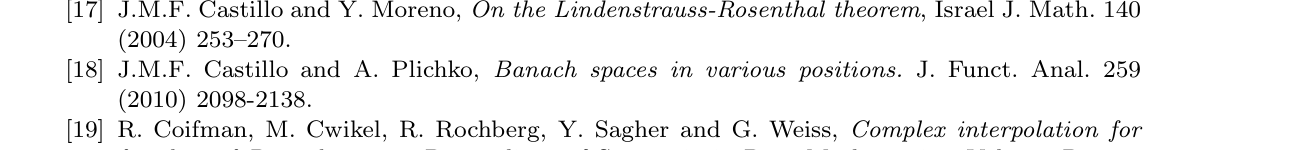
\includegraphics[width=\textwidth]{figures/bibliography_castillo_plichko_crop.png}
\caption{arXiv:1307.4386, bibliography: reference [18] is the
Castillo--Plichko 2010 JFA paper.}
\end{figure}

\section*{Answer recorded in arXiv:1307.4386}

The key passage is in Section 4, ``Counterexamples.'' It recalls the definition
of weak Hilbert spaces, considers Tsirelson's 2-convexified space \(\Ttwo\),
and concludes that not all weak Hilbert spaces are UFO.

\begin{figure}[h]
\centering
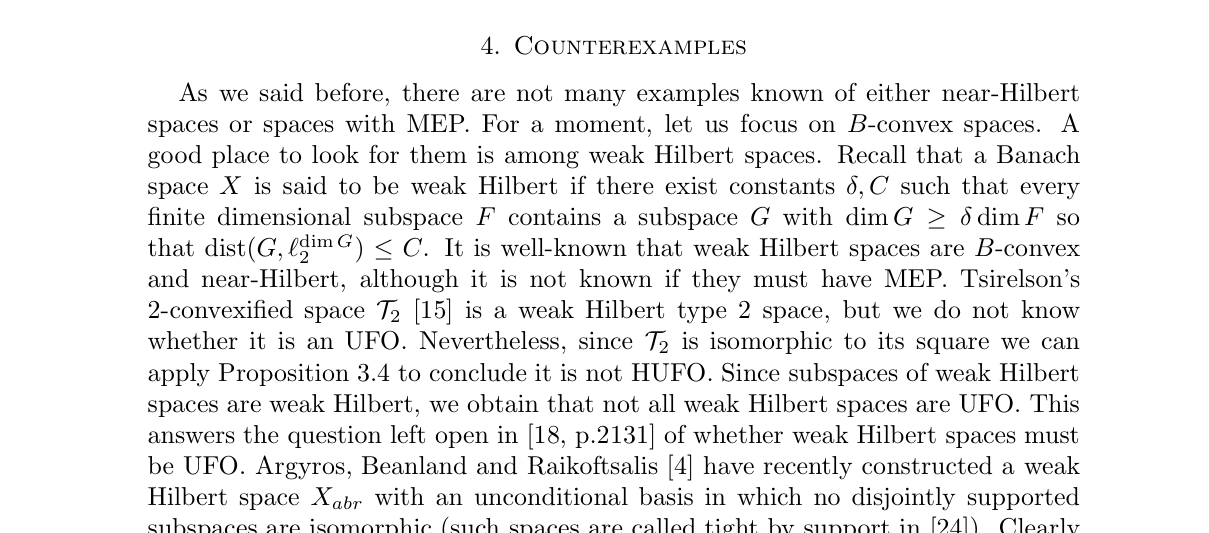
\includegraphics[width=\textwidth]{figures/quoted_question_answer_crop.png}
\caption{arXiv:1307.4386, page 10: the weak-Hilbert counterexample argument
and the explicit statement that the question from [18, p.2131] is answered.}
\end{figure}

\begin{theorem}[Literature status]
There exists a weak Hilbert Banach space which is not UFO. Equivalently, the
question whether weak Hilbert spaces must be UFO has a negative answer.
\end{theorem}

\begin{proof}[Argument as recorded in the answering paper]
The paper uses the following ingredients. First, Tsirelson's 2-convexified
space \(\Ttwo\) is a weak Hilbert type 2 space. Second, \(\Ttwo\) is
isomorphic to its square. Third, Proposition 3.4 of the same paper says that
any HUFO space isomorphic to its square is isomorphic to a Hilbert space.
Since \(\Ttwo\) is not Hilbert, it follows that \(\Ttwo\) is not HUFO.

Now suppose, toward contradiction, that every weak Hilbert space were UFO.
Subspaces of weak Hilbert spaces are weak Hilbert, so every closed subspace of
\(\Ttwo\) would be UFO. That is exactly to say that \(\Ttwo\) would be HUFO,
contradicting the preceding paragraph.

Therefore at least one closed subspace of \(\Ttwo\) is weak Hilbert but not
UFO.
\end{proof}

\section*{What is not being claimed}

The conclusion is existential. It should not be rewritten as ``\(\Ttwo\) is
not UFO.'' The answering paper explicitly says that it does not know whether
\(\Ttwo\) itself is UFO. What it proves is that \(\Ttwo\) is not HUFO, and
hence some weak Hilbert subspace of \(\Ttwo\) fails to be UFO.

This packet is also not a new solution by the present run. It records a
literature answer already stated in arXiv:1307.4386.

\section*{Verification notes and limitations}

Local run-index searches on 2026-06-14 found no prior packet for
arXiv:1307.4386 or for the weak-Hilbert/UFO question. The packet includes the
answering paper and two evidence crops: the answer passage and the
bibliography entry identifying [18].

The original Castillo--Plichko 2010 page 2131 was not acquired during this
loop. Thus the source-question evidence here is the later authors' explicit
citation and description of the question left open in [18, p.2131].

\end{document}
